\documentclass[12pt]{article}

\usepackage{imports/sbc-template}
\usepackage{graphicx, url}
\usepackage{microtype}
\usepackage{amsmath, amsfonts, amssymb}
\usepackage[table,xcdraw]{xcolor}
\usepackage{booktabs, multirow, multicol}
\usepackage{subfig}
\usepackage[utf8]{inputenc}
\usepackage[english]{babel}

\usepackage[inline, shortlabels]{enumitem}

\usepackage{colortbl}
\usepackage{pifont}

\usepackage{pgfplots}
\pgfplotsset{compat=1.9}

\newtheorem{definition}{Definition}

\usetikzlibrary{
    shapes.geometric, patterns
}

% Commands
\newcommand{\todo}[1]{{\color{red}{#1}}}
\newcommand{\thais}[1]{{\color{blue}{#1}}}
\newcommand{\anthony}[1]{{\color{orange}{#1}}}

\newcommand\g{\cellcolor{green!25!white}}
\newcommand\gf[1]{\color{green!80!black}{#1}}
\newcommand\red{\cellcolor{red!25!white}}
\newcommand\rf[1]{\color{red!80!black}{#1}}
\newcommand{\cmark}{\ding{51}}
\newcommand{\xmark}{\ding{55}}

\captionsetup[subfigure]{
  margin=.8cm,
  width=.45\textwidth,
  font=footnotesize,
  format=plain,
  labelfont={bf,sf},
  textfont={bf,sf},
  labelsep=period,
  labelformat=simple
}

\sloppy

\title{Practical algorithms and parameters for \\ modification-tolerant signature scheme}

\author{
    Anthony B. Kamers\inst{1}, Paola de Oliveira Abel\inst{1}, \\
    Thaís B. Idalino\inst{1}, Gustavo Zambonin\inst{1}, Jean E. Martina\inst{1}
}

\address{
    Departamento de Informática e Estatística -- Universidade Federal de Santa Catarina (UFSC)\\
    Caixa Postal 476 -- 88040-370 -- Florianópolis -- SC -- Brazil
    \email{\{anthony.kamers,gustavo.zambonin\}@posgrad.ufsc.br,}
    \email{paola.abel@grad.ufsc.br, \{thais.bardini,jean.martina\}@ufsc.br}
}

\def\instnum{} % Making \instnum empty

\begin{document}

% Variables
\def\floor#1{\lfloor #1 \rfloor}
\def\F{\mathbb{F}}
\def\H{\mathcal{H}}
\def\M{\mathcal{M}}
\def\dRelation{d = \floor{\frac{q-1}{k-1}}}
\def\suchThat{\, |\,}
\def\sk{\mathsf{sk}}
\def\pk{\mathsf{pk}}

\maketitle

\begin{abstract}
  Traditional digital signature schemes are insufficient to identify exactly which part of a signed document had its integrity compromised. In INDOCRYPT '19, Idalino et al. presented an efficient modification-tolerant signature scheme (MTSS) framework using group testing techniques, enabling the detection and correction of modified parts. However, the authors did not give ideal parameters for real use case scenarios. We implement the framework, discuss the practical consequences of the effort, give several parameter sets, and compare the performance of MTSS against traditional signature schemes. We additionally propose a novel use case of the framework, which allows for the integrity of any part of a signed document to be verified without ownership of the whole message.
\end{abstract}

\section{Introduction}
\label{sec:introduction}

A traditional digital signature scheme enables a user to claim the integrity and authenticity of some signed data. The signature verification algorithm has a boolean output, which allows for the \emph{detection} of modifications; it reports failure if a single bit of a signed document is modified. In practical terms, the signer and the information contained within the document may not be trusted. However, if additional properties such as \emph{location} and \emph{correction} of possible modifications~\cite{mtss-idalino-2019} are considered, digital signatures can be employed in a variety of new scenarios.

In \cite{mlss-idalino-2015}, the authors cite several important use cases:
\begin{enumerate*}[(i)]
  \item modification discovery in fillable forms, allowing one to sign the empty form and others to fill it in without invalidating the original signature; 
  \item crime investigations by data forensics, where the investigator may retrieve more information about the attacker by knowing what was modified~\cite{index-data-attacker-goodrich-2005};
  \item improving the efficiency of computer systems: for instance, if we detect where a large database was modified, we do not invalidate it;
  \item privacy protection, where parts of a signed document can be intentionally redacted without invalidating the original signature (cf. content extraction signatures \cite{content-extraction-signature-steinfeld-2002} and redactable signatures \cite{homomorphic-signatures-johnson-2002, redactable-signatures-haber-2008}).
\end{enumerate*}

In the literature, the location property was addressed by~\cite{group-testing-hash-functions-de-bonis-2011,group-testing-hash-functions-de-bonis-2011-2} in the context of hash functions, by~\cite{message-authentication-de-crescenzo-2004,message-authentication-goodrich-2005} in the context of message authentication codes, and by~\cite{mlss-idalino-2015,mtss-idalino-2019} in the context of digital signatures. In general, the authors propose to compute extra integrity information that can be used later for the location of modifications.

There also exist situations where portions of the data can be intentionally removed, redacted, or modified. This is the case of malleable signature schemes, which are studied under the name of \emph{redactable} and \emph{sanitizable} signatures~\cite{position-signatures-bilzhause-2017}. They allow the modification of the signed data in a controlled way (in some cases, by a third party) while the signature is still successfully verified. Such schemes are commonly applied in privacy settings, in which portions of the target data are required to be redacted~\cite{homomorphic-signatures-johnson-2002, redactable-signatures-haber-2008, redactable-signatures-lim-2011}.

Notably, the \emph{modification-tolerant signature scheme} (MTSS) framework employs combinatorial group testing techniques, using \textit{cover-free families} (CFFs), to locate modified parts of a signed document~\cite{mtss-idalino-2019}. Intuitively, a document is split into blocks and grouped according to a CFF on signature generation. When verifying the signed document, the framework allows for the location of modified blocks via the underlying CFF. If the blocks are small enough, it is possible to recover the original file, depending on the parameter choices of the scheme. MTSS can be used with any signature scheme, such as RSA, elliptic curves, or post-quantum algorithms.

We address some open questions of the proposal as laid out in \cite{mtss-idalino-2019}. Namely, we concretely implement MTSS in a high-level programming language and use different underlying signature schemes to measure its performance. We debate which parameters are feasible for constructing CFFs in many scenarios and measure the performance of signature algorithms with such constructions. We also discuss strategies to divide to-be-signed documents into blocks, considering different types of documents and the criteria that affect error identification during signature verification. Additionally, we propose a novel usage of a variation of MTSS that verifies the authenticity and integrity of some parts of a signed document without having access to the entire signed data. Our contributions rely on modification-tolerant signature schemes regarding authentication and data integrity. In this work, we do not explore applications regarding privacy (such as redactable and sanitizable signatures).

This work is organized as follows. In Sect.~\ref{sec:definitions}, we briefly give the necessary background to understand MTSS and our contributions. In Sect.~\ref{sec:discussion-mtss-parameters}, we present our specific objectives and give technical details about the practical implementation of MTSS. In Sect.~\ref{sec:experiments}, we discuss the selection of parameters and other implementation choices for MTSS; we also provide several performance and storage measurements. In Sect.~\ref{sec:partial-data-integrity}, we propose a variation of MTSS that verifies the integrity and authenticity of a single block of the document without having access to the whole document. Finally, in Sect.~\ref{sec:conclusion}, we summarize our contributions and suggest further contributions as future work.

\section{Definitions}
\label{sec:definitions}

% This section covers the definition of cover-free families, followed by the MTSS framework.

\subsection{Cover-free families}
\label{sec:cff}

A set system is a tuple $(X, \mathcal{B})$, where $X$ is a set of points and $\mathcal{B} = \{B_1, \ldots, B_n\}$ is a collection of subsets of $X$, called blocks. Intuitively, a $d$-cover-free family is a set system where the union of any $d$ blocks does not cover any other block in $\mathcal{B}$; a formal definition is given as follows.

\begin{definition}[$d$-CFFs]\label{def:cff}
Let $d, t, n$ be positive integers, with $d < t \leq n$. A $d$-cover-free family, denoted \emph{$d$-CFF($t,n$)}, is a set system $(X, \mathcal{B})$ with $|X| = t$, $|\mathcal{B}| = n$, where for any block $B_{i_0}$ and any other $d$ blocks $B_{i_1}, \ldots, B_{i_d}$ in $\mathcal{B}$ we have $|B_{i_0} \setminus \cup_{j=1}^d B_{i_j}| \geq 1$.
\end{definition}

We may also define a $d$-CFF($t,n$) in terms of its incidence matrix $\M$: a $t \times n$ binary matrix with $\M_{i,j} = 1$ if $x_i \in B_j$, and $0$ otherwise. In the literature, this matrix representation is also known as a $d$-disjunct matrix. We hereafter say a binary matrix is $d$-CFF if its corresponding set system is $d$-CFF. Figure~\ref{fig:example} shows an example of a $2$-CFF($9, 12$) incidence matrix where $X = \{1, \ldots, 9\}$, the collection $\mathcal{B} = \{B_a, B_b, \ldots, B_{l}\}$, and $B_a = \{1,2,3\}, B_b = \{4,5,6\}, \ldots, B_{l} = \{3, 5, 7\}$. CFFs are used in combinatorial group testing, where $n$ items must be tested, and we can detect at most $d$ items as ``defective''. The items are represented by the columns of the incidence matrix $\M$, and the rows identify the groups to be tested. 


%A binary matrix is a $d$-CFF($t,n$) if, for any set of $d+1$ columns, the submatrix indexed by these columns contains a permutation submatrix of order $d+1$.

%Note that if we pick any two columns, all other columns will have at least one ``1" in a row where those two have a ``0".

The $d$-CFF property allows us to perform only $t$ tests and identify up to $d$ defects among the $n$ items in the following way: groups that pass the test contain only non-defective items; the remaining ones are considered defective. 
Figure~\ref{fig:procedure} shows how we can identify up to $2$ defective items using a $2$-CFF($9,12$). Groups $3, 5, 8, 9$ passed the test, and therefore the items in these groups are all non-defective (in green). Groups that fail the test must contain at least one defective item, and so after identifying the non-defective items, the remaining ones are the defective ones (in red). If there are more than $d$ defective items, some non-defective items might be erroneously considered defective due to the group testing technique.

\begin{figure}[htbp]
  \centering
  \subfloat[
    Incidence matrix of a $2$-CFF($9, 12$).
  ]{\label{fig:example}\resizebox{.45\textwidth}{!}{$
  \begin{array}{l|*{12}{l}|}
    \multicolumn{1}{l}{} & a & b & c & d & e & f & g & h & i & j & k & \multicolumn{1}{l}{l} \\
    \cline{2-13}
    1 & 1 & 0 & 0 & 1 & 0 & 0 & 1 & 0 & 0 & 1 & 0 & 0 \\
    2 & 1 & 0 & 0 & 0 & 1 & 0 & 0 & 1 & 0 & 0 & 1 & 0 \\
    3 & 1 & 0 & 0 & 0 & 0 & 1 & 0 & 0 & 1 & 0 & 0 & 1 \\
    4 & 0 & 1 & 0 & 1 & 0 & 0 & 0 & 0 & 1 & 0 & 1 & 0 \\
    5 & 0 & 1 & 0 & 0 & 1 & 0 & 1 & 0 & 0 & 0 & 0 & 1 \\
    6 & 0 & 1 & 0 & 0 & 0 & 1 & 0 & 1 & 0 & 1 & 0 & 0 \\
    7 & 0 & 0 & 1 & 1 & 0 & 0 & 0 & 1 & 0 & 0 & 0 & 1 \\
    8 & 0 & 0 & 1 & 0 & 1 & 0 & 0 & 0 & 1 & 1 & 0 & 0 \\
    9 & 0 & 0 & 1 & 0 & 0 & 1 & 1 & 0 & 0 & 0 & 1 & 0 \\
    \cline{2-13}
    \end{array}
  $}} \hfill
  \subfloat[
    Procedure to identify defects.
  ]{\label{fig:procedure}\resizebox{.52\textwidth}{!}{$
  \begin{array}{l|*{12}{l}|}
    \multicolumn{1}{l}{} & \gf{a} & \gf{b} & \gf{c} & \rf{d} & \gf{e} & \gf{f} & \gf{g} & \rf{h} & \gf{i} & \gf{j} & \gf{k} & \multicolumn{1}{l}{\gf{l}} \\
    \cline{2-13}
    \text{Test 1} \;\rf{\text{\xmark}} & 1 & 0 & 0 & \red 1 & 0 & 0 & 1 & 0 & 0 & 1 & 0 & 0 \\
    \text{Test 2} \;\rf{\text{\xmark}} & 1 & 0 & 0 & 0 & 1 & 0 & 0 & \red 1 & 0 & 0 & 1 & 0 \\
    \text{Test 3} \;\gf{\text{\cmark}} & \g 1 & \g 0 & \g 0 & \g 0 & \g 0 & \g 1 & \g 0 & \g 0 & \g 1 & \g 0 & \g 0 & \g 1 \\
    \text{Test 4} \;\rf{\text{\xmark}} & 0 & 1 & 0 & \red 1 & 0 & 0 & 0 & 0 & 1 & 0 & 1 & 0 \\
    \text{Test 5} \;\gf{\text{\cmark}} & \g 0 & \g 1 & \g 0 & \g 0 & \g 1 & \g 0 & \g 1 & \g 0 & \g 0 & \g 0 & \g 0 & \g 1 \\
    \text{Test 6} \;\rf{\text{\xmark}} & 0 & 1 & 0 & 0 & 0 & 1 & 0 & \red 1 & 0 & 1 & 0 & 0 \\
    \text{Test 7} \;\rf{\text{\xmark}} & 0 & 0 & 1 & \red 1 & 0 & 0 & 0 & \red 1 & 0 & 0 & 0 & 1 \\
    \text{Test 8} \;\gf{\text{\cmark}} & \g 0 & \g 0 & \g 1 & \g 0 & \g 1 & \g 0 & \g 0 & \g 0 & \g 1 & \g 1 & \g 0 & \g 0 \\
    \text{Test 9} \;\gf{\text{\cmark}} & \g 0 & \g 0 & \g 1 & \g 0 & \g 0 & \g 1 & \g 1 & \g 0 & \g 0 & \g 0 & \g 1 & \g 0 \\
    \cline{2-13}
    \end{array}
  $}}
  \caption{Matrix representation of a CFF and defect location procedure. % Adapted from~\cite{tcc-paola}.
  }
  \label{fig:cff-procedure-defects}
\end{figure}

Hence, given $n$ and $d$, we aim to build $d$-CFFs that minimize the number of rows $t$. In the case $d = 1$, an optimal construction is given by Sperner set systems. For a given $n$, we set $t = \min \{s : \binom{s}{\floor{s/2}} \geq n\}$. Then, let $X = \{ 1, 2, \ldots, t\}$ and $\mathcal{B}$ be the collection of all distinct subsets of $X$ of size ${\floor{t/2}}$~\cite{sperner,Wei2006OnFamilies}. Since all subsets are distinct and have the same size, no subset is contained in any other, yielding a $1$-CFF($t,n$).

%With this construction, $t$ grows as $\log_2 n$ as $t \rightarrow \infty$~\cite{?}.

For $d \geq 2$, it is known that $t \geq c\frac{d^2}{\log d } \log n$ for a constant $c$~\cite{Furedi1996OnFamilies,Ruszinko1994OnFamilies,Wei2006OnFamilies}. The best existence results are given by probabilistic methods, achieving $t = \Theta(d^2 \log n)$~\cite{Bshouty2015LinearProblems, Gargano2020Low-weightApplications, Porat2011ExplicitSchemes, Rescigno2022BoundsAlgorithms}. We hereafter consider a polynomial construction based on finite fields, first presented in~\cite{erdos-1985}. 

Consider a finite field $\F_q$, with $q$ a prime power and $2 \leq k \leq q$. We define $\F_q[x]_{<k}$ to be the set of all polynomials with degrees less than $k$ and coefficients in $\F_q$. For $d \leq \floor{\frac{q-1}{k-1}}$, a $d$-CFF($q^2, q^k$) defined by the set system $(X, \mathcal{B})$ is constructed as follows. Let $X = \F_q \times \F_q$; then, for each polynomial $p \in \F_q[x]_{<k}$ we have an associated subset $B_p = \{(a_1, p(a_1)), \dots, (a_q, p(a_q))\}$, and consequently $\mathcal{B} = \{B_p : p \in \F_q[x]_{<k}\}$. For more details on cover-free families, applications, and other constructions for the case $d \geq 2$, see~\cite{survey-cffs}.

\subsection{The modification-tolerant signature scheme framework}
\label{sec:mtss}

As previously mentioned, the MTSS framework \cite{mtss-idalino-2019} is able to locate $d$ modifications in a signed document using a $d$-CFF$(t, n)$. On signature generation, a to-be-signed document must be split into $n$ blocks of $s$ bits to fit the underlying CFF. For blocks of small enough size, the authors also propose correcting such modifications. The signature must carry extra information in the form of cryptographic hashes of blocks in each row (or test). From now on, we may refer to \emph{test} as the document hashes computed using a CFF. Thus, signature size depends on $t, d$, and $n$, and it is crucial to provide parameter sets compatible with several use cases.

Let $\Sigma$ be a digital signature scheme, with the usual key generation (\textsc{KeyGen}), signature generation (\textsc{Sig}), and signature verification (\textsc{Ver}) algorithms; let $\H$ be a cryptographic hash function, and $\M$ a $d$-CFF$(t, n)$ incidence matrix. We hereafter refer to a complete instantiation of the framework as \textsc{MTSS}$(\Sigma, \H, \M)$. MTSS has 4 algorithms: \textsc{KeyGen}, \textsc{Sig}, \textsc{Ver} and ``verify-and-correct'' (\textsc{VCor}); a brief description of each one is given as follows. We also define the set of modified blocks identified by the framework as $I$. Let $\top$ be a valid output, and $\bot$ otherwise.

\noindent \textbf{\textsc{KeyGen}($\lambda$)}. 
Let $\lambda \in \mathbb{N}$ be the security parameter. The algorithm proceeds as follows.
\begin{enumerate}
  \item Set $(\sk, \pk) \leftarrow \Sigma.\textsc{KeyGen}(\lambda)$.
  \item Output $(\sk, \pk)$.    
\end{enumerate}

\noindent \textbf{\textsc{Sig}($m, \sk$)}.
Let $\sk$ be a private key of $\Sigma$, and $m = (m_{1}, \dots, m_{n})$ any message divided into $n$ blocks. The algorithm proceeds as follows.
\begin{enumerate}
  \item\label{sig:1} For $1 \leq i \leq t$ and $1 \leq j \leq n$, set $h_j \leftarrow \H(m_{j})$, $c_i$ the concatenation of all $h_j$ such that $\M_{i,j} = 1$, and $T_{i} \leftarrow \H(c_{i})$.
  \item\label{sig:2} Set $T \leftarrow (T_{1}, \dots, T_{t}, \H(m))$.
  \item\label{sig:3} Set $\sigma' \leftarrow \Sigma.\textsc{Sig}(T, \sk)$.
  \item\label{sig:4} Output $(\sigma', T)$.
\end{enumerate}

\noindent \textbf{\textsc{Ver}($m, \sigma, \pk$)}.
Let $m = (m_{1}, \dots, m_{n})$ be any message divided into $n$ blocks, $\sigma = (\sigma', T)$ a MTSS signature, and $T = (T_{1}, \dots, T_{t}, h_m)$, and $\pk$ a public key of $\Sigma$. The algorithm proceeds as follows.
\begin{enumerate}
  \item\label{ver:1} Set $r \leftarrow \Sigma.\textsc{Ver}(T, \sigma', \pk)$. If $r = \bot$, output $(\bot, \{\})$. Otherwise, go to step~\ref{ver:2}.
  \item\label{ver:2} If $\H(m) = h_m$, output $(\top, \{\})$. Otherwise, go to step~\ref{ver:3}.
  \item\label{ver:3} For $1 \leq i \leq t$, compute $T'_{i}$ analogously to Step~\ref{sig:1} of \textsc{Sig}.
  \item\label{ver:4} Set $V \leftarrow \{\}$. For $1 \leq i \leq t$, if $T_{i} = T'_{i}$, set $V \leftarrow V \cup \{j : \M_{i,j} = 1\}$.
  \item\label{ver:5} Set $I \leftarrow \{1, \dots, n\} \setminus V$. If $|I| \leq d$, output $(\top, I)$; otherwise, output $(\bot, I)$.
\end{enumerate}

\noindent \textbf{\textsc{VCor}($m, \sigma, \pk$)}. 
Let $m = (m_{1}, \dots, m_{n})$ be any message divided into $n$ blocks, $\sigma = (\sigma', T)$ a MTSS signature, and $\pk$ a public key of $\Sigma$. The algorithm proceeds as follows.
\begin{enumerate}
  \item\label{vcor:1} Set $(r, I) \leftarrow \textsc{Ver}(m, \sigma, \pk)$. If $r = \bot$, output $(\bot, \{\}, \{\})$. Otherwise, go to step~\ref{vcor:1.5}.
  \item\label{vcor:1.5} If $|I| = 0$, go to step~\ref{vcor:6}. Otherwise, set $b \leftarrow \min(I)$, $I \leftarrow I \setminus b$ and go to step~\ref{vcor:2}.
  \item\label{vcor:2} Set $i$ to be the index of any row $\M_{i}$ such that $\M_{i,b} = 1$ and $\M_{i,j} = 0$ for all $j \in I$.
  \item\label{vcor:3} For all $j$ such that $\M_{i,j} = 1$ and $j \neq b$, set $h_{j} \leftarrow \H(m_{j})$. Set $c_{b} = \bot$.
  \item\label{vcor:4} For every possible bit string $q$ of size $\leq s$:
    \begin{enumerate}
      \item Set $h_b \leftarrow \H(q)$.
      \item For $1 \leq j \leq n$, compute $T'_{i}$ analogously to Step~\ref{sig:1} of \textsc{Sig}.
      \item If $T'_{i} = T_{i}$ and $c_{b} = \bot$, set $c_{b} = \top$ and $m_{b} \leftarrow q$; otherwise, if $T'_{i} = T_{i}$ and $c_{b} = \top$, output $(\top, I, \varepsilon)$, where $\varepsilon$ is the empty string.
    \end{enumerate}
  \item\label{vcor:5} Go to step~\ref{vcor:1.5}.
  \item\label{vcor:6} Output $(\top, I, m)$.
\end{enumerate}

We refer the reader to~\cite{mtss-idalino-2019} for a detailed algorithm explanation and proof of the security and correctness of the framework. We remark on an interesting characteristic of MTSS: given only a signature $\sigma$ and the number of blocks $n$, we can reconstruct $\M$. This may be used for implementation purposes. In the following, we address the practical consequences of the algorithms above, such as the division of $m$ into $n$ blocks, the construction of $\M$, and the impact of $\Sigma$, $\H$, and the aforementioned procedures in overall performance and signature sizes.

\section{Discussion on MTSS parameters}
\label{sec:discussion-mtss-parameters}

As previously mentioned, several practical considerations were not given or deeply explored in \cite{mtss-idalino-2019}. We present the following questions as a guideline for our discussion about parameters and their consequences on implementations of MTSS.

\begin{enumerate}[label=$\mathbf{Q_{\arabic*}}$, itemsep=.5em, wide, labelindent=0pt, listparindent=0pt]
  \item\label{question:message-blocks}
  
  \emph{How to efficiently implement message division, and what are the consequences for \textsc{Sig}, \textsc{Ver}, and \textsc{VCor}?} 
  
  \vspace{.5em}
  We recall that all algorithms except \textsc{KeyGen} expect to receive a message $m$ already separated in $n$ blocks; however, in practice, a user expects to simply input the entire to-be-signed message, and an implementation of MTSS performs the appropriate division. Hence, we define a \textsc{DivideBlocks($m'$)} algorithm, which separates the input message $m'$ into blocks according to some criteria depending on the file type. Its output is a tuple $(m, n)$, where $m = (m_{1}, \dots, m_{n})$. Our implementation does not consider $n$ as a free input because of possible issues in locating errors using \textsc{Ver} algorithm; rather, we infer $n$ from the type of document chosen. We further address this question in Sections~\ref{sec:documents-blocks-distribution} and~\ref{sec:auxiliary-algorithms}.

  \item\label{question:cff-parameters}

  \emph{Which parameters are suitable for $\M$ and what is their effect on performance?} 
  
  \vspace{.5em}
  As per Sect.~\ref{sec:cff}, a CFF is defined via parameters $d, t$, and $n$, with $t$ minimized. We recall that $n$ is the number of blocks of a message $m'$ given by \textsc{DivideBlocks}($m'$), as discussed in~\ref{question:message-blocks}. It remains to calculate $d$ and $t$; we recall that the parameter $k$ can be used to yield $d$ and $t$, and also $q$ for $k \geq 2$, via the constructions presented in Sect.~\ref{sec:cff}. Hence, we define the \textsc{CreateCFF($n, k$)} algorithm as follows: if $k = 1$, the Sperner construction is used, where $d = 1$; otherwise, we use the polynomial over finite fields construction, in which $d$ depends on $q$ and $k$, i.e., given $n$ and $k$, we choose the smallest $q$ such that $n \leq q^k$. Its output is the incidence matrix $\M$. We further address this question in Sections \ref{sec:cff-parameters} and~\ref{sec:auxiliary-algorithms}.

  \item\label{question:hash-choice}

  \emph{How does the choice of $\H$ impact overall performance?}

  \vspace{.5em}
  We observe that \textsc{Sig} and \textsc{Ver} require $nt + 1$ evaluations of $\H$. Thus, the choice of the underlying cryptographic hash function greatly influences the performance of operations on signatures. We evaluate several choices of $\H$, and give performance results and recommendations in Sections \ref{sec:signature} and~\ref{sec:verification}.

  \item\label{question:sigma-choice}

  \textit{How does the choice of $\Sigma$ impact overall performance?}

  \vspace{.5em}
  We observe that the authors of~\cite{mtss-idalino-2019} roughly estimate the performance of MTSS depending on $\Sigma$. We explore other choices of signature schemes and give actual performance and signature size results in Sections \ref{sec:signature} and~\ref{sec:verification}.
\end{enumerate}

\subsection{Documents and blocks division}
\label{sec:documents-blocks-distribution}

We remark that CFF blocks need not be homogeneous in size; this is useful for digital documents since each file type has specific syntactic characteristics. However, as per Step~\ref{vcor:4} of the \textsc{VCor} algorithm, a large block implies a slower error correction procedure since all possible bit strings need to be searched to correct the block. Hence, efficient block division criteria are relevant in this context. Several authors \cite{mtss-idalino-2019, different-data-structures-pohls-2018} consider strategies such as sequential ordering considering some delimiter, non-sequential ordering using complex structural data, a header at the beginning of the file informing the blocks, or even a combination of these.

The easiest way to separate the content into blocks is to divide a message into sequential sections of fixed size. However, this approach is not free of problems~\cite{mlss-idalino-2015}. Without loss of generality, for any bit string that is divided into blocks, if any bit is added to or removed from any block but the last, a cascade effect happens to the subsequent blocks. To prevent this problem, we must define document representations and block delimiters for the \textsc{DivideBlocks} algorithm. 

We first consider plain text files using the ASCII encoding; we set the line break (\texttt{0x0a}) character as the default delimiter. Hence, the number of lines must remain the same to detect changes, but any individual lines are modifiable. We also discuss how to interpret XML files (also encoded in ASCII) as an example of a more complex document type. As canonicalization algorithms usually remove indentation and spaces~\cite{w3-canonicalization-2008}, such characters cannot be used as block delimiters.

The \textit{\textless} (\texttt{0x3c}) character can be used as a delimiter, but we would have redundancy among different types of tags (opening and closing). Hence, we choose to pair opening and closing tags in the same block. The parent tag is kept in a separate block if any child elements exist. One disadvantage of this approach is the excess of usual tag delimiter characters since they are always put in the blocks. This approach can also be applied to other similar markup systems, such as HTML.

A more natural way for hierarchy file types could be using a tree as structural data. This way, we could separate each node as a tag and their children as connected to this parent node. This separation method could also be used for other hierarchy-like files. Nevertheless, we show hereafter that the \textsc{DivideBlocks} algorithm has poor efficiency using the simple pair opening and closing tags, and using a tree would add more complexity to that. Besides, we would have the override of implementing a search algorithm to access a particular node, which would also affect the performance of MTSS algorithms.

% This method decreases the size of blocks since it does not need the auxiliary characters; besides, it would be possible to sign and validate documents whose order would not matter, like database queries; if the order is necessary, we could make a binary tree with search algorithms or labeled attributes in each node.

\subsection{CFF parameters}
\label{sec:cff-parameters}

We remark some initial observations from the algorithms described in Sect.~\ref{sec:mtss}:
\begin{enumerate*}[(i)]
  \item the signature size grows with the number of blocks $n$;
  \item to efficiently correct modifications, it is suggested to limit block size to a small enough size $s$. However, this minimization leads to more blocks;
  \item larger blocks lead to less accuracy in error location and fewer tests $t$ executed.
\end{enumerate*}
In this context, we aim to find ideal parameters for polynomial constructions, i.e., $d \geq 2$. From Sect.~\ref{sec:cff}, we recall that $n = q^k$ or $n = t^{k/2}, t = q^2$, and $d \leq \floor{\frac{q-1}{k-1}}$. As previously mentioned, we calculate $q$ from $n$ and $k$ via the \textsc{CreateCFF} algorithm. 

To generate smaller CFFs and improve efficiency, we increase the gap between the number of blocks and tests to minimize $t$. The proportion between $n$ and $t$ is given by $q^{k - 2}$, which gives us the signature compression rate; hence, larger values for $k$ lead to further gains in compression. However, due to the upper bound of $d$, we observe that smaller $k$ are useful for achieving larger error location abilities. On the other hand, $q \leq 5$ are not generally useful because they generate $1$-CFFs, which are already optimally built using Sperner set systems. The same occurs for $k \geq 7$ since most constructions with this parameter can be achieved via Sperner families or are meant for larger $n$.

A $d$-CFF($q^2, q^k$) allows locating up to $d$ modifications. The ratio between $d$ and $n$ is given as follows: $\frac{d}{n} = \frac{(q-1)/(k-1)}{q^k}$. This leads us to a conclusion: for fixed $n$, smaller values of $q$ have a better proportion of modifiable blocks $d$. Furthermore, the aforementioned relation between $d, q$, and $k$ shows that $d$ grows with $q$. These statements help us answer \ref{question:cff-parameters}. In summary, smaller values for $k$ have more advantages: they optimize the modification localization while obtaining modifiable blocks at a higher number and proportion. Hence, we suggest $3 \leq k \leq 7$ and $q > 5$ to yield efficient constructions when $d \geq 2$.


% We additionally observe the percentage of modified blocks of a $d$-CFF($q^2, q^k$) is given by $\thais{\frac{d}{n}} = \frac{(q-1)/(k-1)}{q^k}$.

\section{Experiments}
\label{sec:experiments}

We provide an open-source implementation\footnote{\url{https://github.com/AnthonyKamers/mtss-signer/}} of the MTSS framework as described in the original work~\cite{mtss-idalino-2019}. We use Python 3.10 and run the tests on an Intel Core i7-13700H @ 5.0 GHz with CPU performance scaling disabled. Except when otherwise indicated, the performance results presented in this section were calculated by executing each algorithm 100 times and taking the mean. For the choices of $\Sigma$, we consider
\begin{enumerate*}[(i)]
  \item RSA-2048 and RSA-4096, which are known to be widely used in public-key cryptographic applications~\cite{rsa-most-used-cao-2008};
  \item Ed25519, an elliptic-curve signature scheme which is a recent alternative to RSA, with smaller signatures and higher overall performance~\cite{ed25519-bernstein-2012};
  \item and all instances of ML-DSA, a post-quantum algorithm based on lattices which is currently in the process of standardization by the U.S. National Institute of Standards and Technology~\cite{fips-204-dilithium-nist-2023}.
\end{enumerate*}

We also consider several cryptographic hash functions for the choice of $\H$: SHA2-256, SHA2-512, SHA3-256, SHA3-512, BLAKE2s, and BLAKE2b. We argue that these choices of $\Sigma$ and $\H$ represent a wide range of use cases and allow for easier reproducibility of our results while also considering state-of-the-art algorithms. We note that $\H$ may vary according to $\Sigma$, except in the case of Ed25519, where it is required that $\H =$ SHA2-512~\cite{rfc-8032-ed25519}). Otherwise, we test all $\H$ against all $\Sigma$ to compare the performance of signature generation and verification in the context of MTSS.

We follow the guidelines of the original authors of MTSS in our implementation. Particularly, we parallelize hash computations whenever possible in \textsc{VCor}. We anticipate that CFF generation is costly when on-demand, i.e., in every computation of \textsc{Sig}, and if errors are detected by \textsc{Ver}. Therefore, we implement a simple cache for $d$-CFF($t, n$) with distinct $d, t, n$ to prevent such overhead. In our experiments, we assume that all CFFs used are already cached and previously serialized to memory, except when otherwise noted. Finally, we execute \textsc{DivideBlocks} before every computation of \textsc{Sig}, \textsc{Ver}, and \textsc{VCor}.

\subsection{Auxiliary algorithms}
\label{sec:auxiliary-algorithms}

As previously mentioned, auxiliary algorithms for MTSS create overhead in signature generation and verification. In the following, we answer~\ref{question:message-blocks} and~\ref{question:cff-parameters} by respectively discussing the practical consequences of implementing \textsc{DivideBlocks} and \textsc{CreateCFF}. Due to time constraints, both algorithm's performance tests were executed only once.

\begin{figure}[htbp]
    \centering
    \subfloat[Performance of \textsc{DivideBlocks}.]{
        \label{fig:divide-blocks-efficiency}
        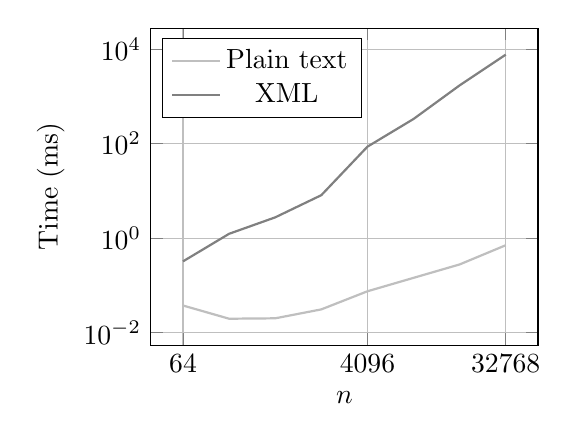
\begin{tikzpicture}
    \begin{semilogyaxis}[
        % title={DivideBlocks algorithm efficiency},
        xlabel={$n$},
        ylabel={Time (ms)},
        legend pos=north west,
        grid=major,
        % width=7cm,
        % height=5cm,
        width=6.5cm,
        log basis x={10},
        xtick={1, 5, 8},
        xticklabels={64,4096,32768}
    ]
    \addplot[
        color=lightgray,
        mark=none,
        thick
        ] coordinates {
        (1, 0.037700000000000004)
        (2, 0.0198)
        (3, 0.020200000000000003)
        (4, 0.031200000000000002)
        (5, 0.07540000000000001)
        (6, 0.1451)
        (7, 0.2788)
        (8, 0.7108)
    };
    \addlegendentry{Plain text}
    
    \addplot[
        color=gray,
        mark=none,
        thick
        ] coordinates {
        (1, 0.32380000000000003)
        (2, 1.2419)
        (3, 2.7662)
        (4, 8.1549)
        (5, 86.5322)
        (6, 334.07800000000003)
        (7, 1718.2588)
        (8, 7686.303800000001)
    };
    \addlegendentry{XML}
    
    \end{semilogyaxis}
\end{tikzpicture}
    }
    \hfill
    \subfloat[Performance of \textsc{CreateCFF}.]{
        \label{fig:cff-polynomial-performance}
        \begin{tikzpicture}
  \begin{axis}[
        xlabel={$q$},
        ylabel={$k$},
        zlabel={Time (ms)},
        zmode=log,
        grid=major,
        xtick={2, 5, 7, 8, 9, 11, 13, 16},
        ytick={2, 3, 4, 5},
        % width=7cm,
        % height=5cm,
        width=6.7cm,
        view={330}{30}
    ]
    \addplot3 [mesh, color=gray] gnuplot [raw gnuplot] {
      set dgrid3d 20, 20, 20;
      splot 'charts/q-k-cff.txt' using 1:2:3 with lines
    };
  \end{axis}
\end{tikzpicture}
    }
    \caption{General performance of auxiliary algorithms for several choices of $k, q, n$.}
\end{figure}

\textbf{Document division}. Figure \ref{fig:divide-blocks-efficiency} summarizes the performance of \textsc{DivideBlocks} considering plain text and XML documents of several sizes. As $n$ increases, XML files require more time to separate into blocks due to the additional overhead of canonicalization, syntactic validation, and structure parsing. However, according to \cite{xml-statistics-mlynkova-2006}, the average size of XML documents is around 4.6 kB, containing a small number of nodes; moreover, 99\% of XML documents have fewer than eight levels. This suggests that, despite larger XML documents taking longer to separate into blocks, most real-world XML documents are relatively short and simple, making them suitable for use with MTSS in practical applications. Nonetheless, since parsing plain text files is considerably simpler, our subsequent experiments will focus on this file type.

\textbf{CFFs}. We first note that, for a fixed number of blocks $n$, the relative number of tests $t$ is $\approx 173.39\%$ larger when employing polynomial constructions and takes $\approx 2000 \times$ longer to execute. Thus, for the case $d = 1$, Sperner families are the most efficient solution. However, we recall that the polynomial construction is required if $d \geq 2$. Figure~\ref{fig:cff-polynomial-performance} shows the performance of creating CFFs with polynomial constructions for several choices of $k$ and $q$. We observe that as $q$ increases, the execution becomes exponentially slower since $n = q^k$ and, as $n$ grows, the entire CFF grows. A particularly efficient point is shown between $5 \leq q \leq 8$, and $k = 5$, where the parameters are among the ones proposed in Sect.~\ref{sec:cff-parameters}, generates a large CFF and in a reasonable time ($< 40$ms).

While $q > 5$ produces more valuable CFFs, performance tends to decline for values greater than this threshold. Techniques such as pre-constructing the CFFs can mitigate this issue and improve the framework's overall efficiency. If we consider using MTSS in a central resourceful server, CFFs could be made in advance and stored locally, which would not disturb other algorithms' performance.

\subsection{Signing}
\label{sec:signature}

We divide the overall signature generation procedure into two separate stages, \textit{pre-sign} and \textit{sign} (\textsc{Sig} proper), for ease of discussion. In the \textit{pre-sign} stage, we handle I/O operations, segment the message into blocks based on the document type using \textsc{DivideBlocks}, and create or parse the cached CFF with \textsc{CreateCFF}. We integrate both algorithms in the \textit{pre-sign} stage. As a practical consequence, the implementation of \textsc{Sig} takes an additional parameter $k$ so that auxiliary algorithms need not be invoked by the user.

During the \textit{pre-sign} stage, the document $m'$ (not parsed into blocks yet) is read from the disk, processed by \textsc{DivideBlocks($m'$)}, and subsequently by \textsc{CreateCFF($n, k$)}. The secret key $\sk$ is also retrieved from the disk, preparing all necessary components for the \textit{sign} stage. Given the potential computation cost of these operations, we provide examples illustrating the execution time of both stages in the following.

The hash function $\H$ and the signature scheme $\Sigma$ used in the framework significantly impact the signing performance. Table~\ref{table:performance-signature-traditional-mtss} shows a performance comparison of different signature schemes and hash functions in the context of our implementation. We do not consider the \textit{pre-sign} stage in performance measurements. The last two columns represent the size of the resulting MTSS signature in bytes, depending on the output size (in bits) of $\H$. This comparison addresses \ref{question:hash-choice}, demonstrating that the choice of the hash function $\H$ plays a crucial role in MTSS performance. Furthermore, the signing time of MTSS-augmented $\Sigma$ remains consistent with traditional $\Sigma$, which answers \ref{question:sigma-choice}.

\begin{table}[ht]
  \setlength{\tabcolsep}{5.75pt}
  \centering
  \caption{Performance and output size of \textsc{MTSS}($\Sigma, \H, \M$).\textsc{Sig} for several choices of $\Sigma$, $\H$ and security parameter $\lambda$, considering $\M = 2$-CFF($25, 125$), $k = 3$ and a 1.19MB plain text file as input.}
  \begin{tabular}{crlrrrrrrrr}
    \toprule
    &
    \multicolumn{1}{r}{\multirow{5}{*}{$\lambda$}}
        & \multicolumn{1}{c}{\multirow{5}{*}{$\Sigma$}}
        & \multicolumn{6}{c}{\textsc{Sig} time (ms)}
        & \multicolumn{2}{c}{\multirow{3}{*}{$|\sigma|$ (bytes)}} \\
    \cmidrule{4-9}
    & &
        & \multicolumn{2}{c}{SHA-2}
        & \multicolumn{2}{c}{SHA-3}
        & \multicolumn{2}{c}{BLAKE}
        & \\
    \cmidrule{4-11}
    & & & 256 & 512 & 256 & 512 & 2s & 2b & 256 & 512 \\
    \cmidrule{2-11}
    \multirow{6}{*}{\rotatebox[origin=c]{90}{Raw $\Sigma$}}
    & 128 & RSA-2048         & 4.83 & 3.63 & 3.93 & 6.42 & 2.49 & 3.32 & 256  & 256  \\
    & 128 & ML-DSA-44        & 3.93 & 2.67 & 2.96 & 5.49 & 1.54 & 2.36 & 2360 & 2360 \\
    & 128 & Ed25519          &      & 3.08 &      &       &      &      &      & 64   \\
    & 256 & RSA-4096         & 8.83 & 7.64 & 7.96 & 10.44 & 6.54 & 7.38 & 512  & 512  \\
    & 256 & ML-DSA-65        & 3.98 & 2.71 & 2.98 & 5.55 & 1.60 & 2.49 & 3220 & 3220 \\
    & 512 & ML-DSA-87        & 4.10 & 2.73 & 3.02 & 5.58 & 1.62 & 2.41 & 4490 & 4490 \\
    \cmidrule{2-11}
    \multirow{6}{*}{\rotatebox[origin=c]{90}{\textsc{MTSS}}} 
    & 128 & RSA-2048         & 27.35 & 19.42 & 21.76 & 36.85 & 10.86 & 15.63 & 1088 & 1880  \\
    & 128 & ML-DSA-44        & 26.44 & 18.85 & 21.27 & 36.04 & 10.36 & 15.2 & 3180 & 3990  \\
    & 128 & Ed25519          &       & 19.99 &       &       &       &       &      & 1690  \\
    & 256 & RSA-4096         & 31.32 & 23.37 & 25.74 & 40.87 & 14.9 & 19.66 & 1310 & 2120  \\
    & 256 & ML-DSA-65        & 26.63 & 18.83 & 21.1 & 35.93 & 10.22 & 15.29 & 4030 & 4840  \\
    & 512 & ML-DSA-87        & 26.76 & 18.98 & 21.12 & 36.17 & 10.02 & 15.05 & 5300 & 6110  \\
    \bottomrule
  \end{tabular}
  \label{table:performance-signature-traditional-mtss}
\end{table}

Based on these findings, we hereafter consider $\Sigma =$ RSA-2048 and $\H =$ BLAKE2b for our next experiments, as RSA-2048 is commonly used in practice and BLAKE2b showed the best performance among the evaluated hash functions. The performance of \textit{sign} is influenced by the number of tests $t$ in $\M$. We identify that increasing the number of tests results in longer signing times and larger signatures, as shown in Table~\ref{table:sign-locate-different-parameters}. The upper group demonstrates how performance is affected by the size of the input file for fixed $k$. On the other hand, the lower group shows how different $k$ affects the same file. It is important to note that the same file can have varying numbers of tests $t$, depending on the chosen values for $k$. The framework efficiency is reduced as tests or the number of blocks increases. However, MTSS creates stronger signatures that make it easier to identify document alterations, which is crucial in the discussed scenarios.

\begin{table}[htbp]
  \setlength{\tabcolsep}{10pt}
  \centering
  \caption{Performance of signature operations of MTSS($\Sigma, \H, \M$) for several choices of $\M$, plain text files of different sizes, and $|I| = 1$.}
  \begin{tabular}{rrrrrrrrr}
    \toprule
    \multicolumn{5}{c}{Parameters of $\M$} & \multicolumn{2}{c}{Size  (kB)} & \multicolumn{2}{c}{Time (ms)} \\
    \cmidrule(lr){1-5} \cmidrule(lr){6-7} \cmidrule(lr){8-9}
    $k$ & $q$ & $t$ & $n$ & $d$ & $m$ & $\sigma$ & \textsc{Sig} & \textsc{Ver} \\
    \midrule
    4 & 7  & 49   & 2401  & 2  & 4.69 & 3.38 & 56.98   & 33.41   \\
    4 & 9  & 81   & 6561  & 2  & 12.8 & 5.38 & 156.27  & 185.95  \\
    4 & 11 & 121  & 14641 & 3  & 28.6 & 7.88 & 471.47  & 777.91  \\
    4 & 13 & 169  & 28561 & 4  & 55.8 & 10.9 & 1318.92 & 2609.34 \\
    \midrule
     - &  -  & 15   & \multirow{4}{*}{4096}  & 1  & \multirow{4}{*}{8}    & 1.25 & 96.21   & 88.41   \\
    4 & 8  & 64   &   & 2  &    & 4.31 & 91.30   & 82.93   \\
    3 & 16 & 256  &   & 7  &    & 16.3 & 187.37  & 191.41  \\
    2 & 64 & 4096 &   & 63 &    & 256  & 1720.94 & 2238.13 \\
    \bottomrule
  \end{tabular}
  \label{table:sign-locate-different-parameters}
\end{table}

The \textit{pre-sign} stage can sometimes take longer than \textit{sign}, depending on the input file (and subsequent number of blocks). As discussed in Sect.~\ref{sec:auxiliary-algorithms}, parsing large XML files can be time-consuming. This is an important consideration when using the MTSS framework. Figure \ref{fig:performance-sign-algorithm} compares the performance of the \textit{pre-sign} and \textit{sign} stages, showing the total time to sign different files with $k = 4$. For simplicity, each file is named \texttt{n.ext}, where $n$ is the number of blocks and \texttt{ext} represents plain text and XML files. When considering complex files, we note that \textit{pre-sign} can overtake the \textit{sign} stage time.

\begin{figure}[ht]
    \centering
    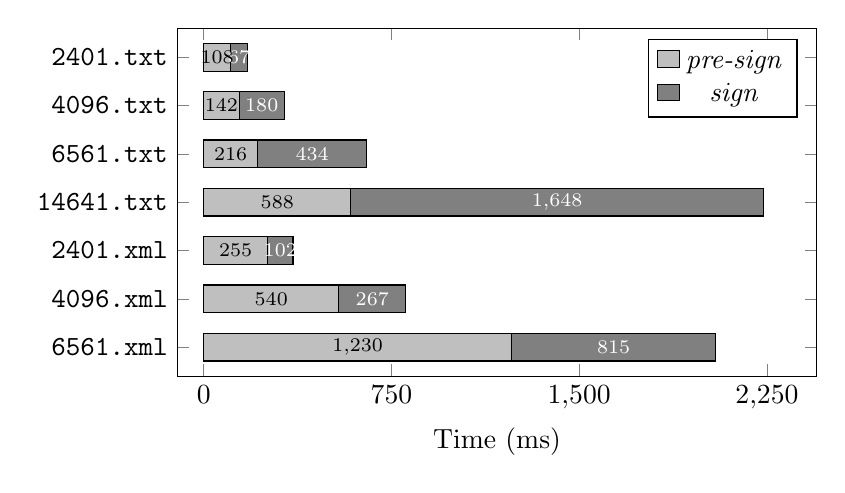
\begin{tikzpicture}
    \begin{axis}[
        width=.8\textwidth,
        height=6cm,
        xbar stacked,
        nodes near coords,
        legend pos=north east,
        xlabel={Time (ms)},
        xtick={0, 750, 1500, 2250},
        symbolic y coords = {
            6561.xml,
            4096.xml,
            2401.xml,
            14641.txt,
            6561.txt,
            4096.txt,
            2401.txt,
        },
        ytick=data,
        y tick label style={font=\ttfamily},
        nodes near coords style={black, font=\scriptsize}
    ]
        \addplot+[
            xbar,
            black,
            fill=lightgray,
        ] plot coordinates {
            (108,2401.txt)
            (142,4096.txt)
            (216,6561.txt)
            (588,14641.txt)
            (255,2401.xml)
            (540,4096.xml)
            (1230,6561.xml)
        };
        \addlegendentry{\textit{pre-sign}}
        
        \addplot+[
            xbar,
            black,
            fill=gray,
            nodes near coords style={white, font=\scriptsize},
        ] plot coordinates {
            (67,2401.txt)
            (180,4096.txt)
            (434,6561.txt)
            (1648,14641.txt)
            (102,2401.xml)
            (267,4096.xml)
            (815,6561.xml)
        };
        \addlegendentry{\textit{sign}}
    \end{axis}
\end{tikzpicture}
    \caption{Performance of the signature generation procedure stages for MTSS($\Sigma, \H, \M$), where $\M$ changes according to each file.}
    \label{fig:performance-sign-algorithm}
\end{figure}

\subsection{Verifying the signature and locating errors}
\label{sec:verification}

Analogously, we divide the signature verification procedure into \textit{pre-verify} and \textit{verify}. The former handles I/O operations by reading the message $m$, signature $\sigma$, and public key $\mathsf{pk}$ from the disk; the latter follows the MTSS \textsc{Ver} algorithm. In the framework, signature verification performance depends on whether the signed message was modified or not. If its integrity is preserved, the efficiency of \textsc{Ver} is comparable to $\Sigma.\textsc{Ver}$, albeit with the overhead of the MTSS signature being larger (cf. $|\sigma|$ in Table~\ref{table:performance-signature-traditional-mtss}). Therefore, we focus on the performance of locating modifications in signed messages.

We discuss the influence of the number of tests $t$ in modified signed messages in Table~\ref{table:sign-locate-different-parameters}. We infer that the verification time is directly proportional to $t$. In order to become practical, fewer tests are desired; nevertheless, depending on the framework's application, more tests and a higher number of modifications detected are expected. This tradeoff is necessary for the more powerful signatures MTSS produces. Another experiment we conducted was changing the number of modified characters $|I|$ in the same document from the bottom part of Table~\ref{table:sign-locate-different-parameters}, using $k = 3$, i.e., generating a $7$-CFF($256, 4096$); we noted that the performance for different $|I|$ is very small, since step \ref{ver:4} from \textsc{Ver} recognizes all modified blocks in a loop, not stopping until reaches all tests.

Table~\ref{table:performance-verify-traditional-mtss} shows the performance overhead of MTSS.\textsc{Ver} with $|I| = 0$ and $|I| = 1$ against verifying using only $\Sigma.\textsc{Ver}$. We remark that locating errors increases the verifying time by up to $2 \times$, depending on the number of tests $t$. However, we still consider it as efficient and practical in real scenarios. This comparison also addresses \ref{question:hash-choice} and \ref{question:sigma-choice} in the context of signature verification.

\begin{table}[ht]
  \setlength{\tabcolsep}{7pt}
  \centering
  \caption{Performance and output size of \textsc{MTSS}($\Sigma, \H, \M$) \textsc{Ver} for several choices of $\Sigma$, $\H$ and security parameter $\lambda$, considering $\M = 2$-CFF($25, 125$), $k = 3$ and a 1.19MB plain text file as input.}
  \begin{tabular}{crlrrrrrr}
    \toprule
    &
    \multicolumn{1}{r}{\multirow{5}{*}{$\lambda$}}
        & \multicolumn{1}{c}{\multirow{5}{*}{$\Sigma$}}
        & \multicolumn{6}{c}{\textsc{Ver} time (ms)} \\
    \cmidrule{4-9}
    & &
        & \multicolumn{2}{c}{SHA-2}
        & \multicolumn{2}{c}{SHA-3}
        & \multicolumn{2}{c}{BLAKE} \\
    \cmidrule{4-9}
    & & & 256 & 512 & 256 & 512 & 2s & 2b \\
    \cmidrule{2-9}
    \multirow{6}{*}{\rotatebox[origin=c]{90}{Raw $\Sigma$}}
    & 128 & RSA-2048         & 4.09 & 2.87 & 3.15 & 5.66 & 3.21 & 4.84   \\
    & 128 & ML-DSA-44        & 3.88 & 2.61 & 2.90 & 5.47 & 1.51 & 2.30   \\
    & 128 & Ed25519          &      & 3.84 &      &      &      &        \\
    & 256 & RSA-4096         & 4.37 & 3.17 & 3.44 & 5.94 & 3.50 & 5.12   \\
    & 256 & ML-DSA-65        & 3.91 & 2.62 & 2.92 & 5.47 & 1.51 & 2.32   \\
    & 512 & ML-DSA-87        & 3.91 & 2.64 & 2.94 & 5.49 & 1.53 & 2.34   \\
    \cmidrule{2-9}
    \multirow{6}{*}{\rotatebox[origin=c]{90}{\textsc{MTSS} ($|I| = 0$)}}
    & 128 & RSA-2048         & 4.16 & 2.95 & 3.25 & 5.80 & 1.81 & 2.64  \\
    & 128 & ML-DSA-44        & 3.94 & 2.69 & 3.00 & 5.55 & 1.55 & 2.37  \\
    & 128 & Ed25519          &      & 3.90 &      &      &      &       \\
    & 256 & RSA-4096         & 4.45 & 3.23 & 3.54 & 6.08 & 2.10 & 2.91  \\
    & 256 & ML-DSA-65        & 3.95 & 2.70 & 3.08 & 5.58 & 1.56 & 2.38  \\
    & 512 & ML-DSA-87        & 3.95 & 2.72 & 3.05 & 5.57 & 1.58 & 2.40  \\
    \cmidrule{2-9}
    \multirow{6}{*}{\rotatebox[origin=c]{90}{\textsc{MTSS} ($|I| = 1$)}} 
    & 128 & RSA-2048         & 159.95 & 174.53 & 162.22 & 162.29 & 153.15 & 162.94   \\
    & 128 & ML-DSA-44        & 156.93 & 177.55 & 159.49 & 165.35 & 163.51 & 154.37   \\
    & 128 & Ed25519          &       & 165.41 &      &       &      &        \\
    & 256 & RSA-4096         & 169.32 & 153.97 & 166.26 & 161.66 & 167.44 & 160.91   \\
    & 256 & ML-DSA-65        & 160.05 & 191.31 & 165.23 & 162.47 & 154.52 & 160.33   \\
    & 512 & ML-DSA-87        & 158.34 & 162.69 & 167.37 & 158.83 & 162.81 & 152.57   \\
    \bottomrule
  \end{tabular}
  \label{table:performance-verify-traditional-mtss}
\end{table}

\subsection{Correcting}
\label{sec:correction}

The \textsc{VCor} algorithm supersets \textsc{Ver}: modified blocks are first located, and then corrections are tried. As mentioned in Sect.~\ref{sec:mtss}, we need to brute-force all possibilities from some block considering some character encoding. Aspects such as the number of blocks, number of modifications, content to be corrected, and the cryptographic hash function used affect the performance of the algorithm. Particularly, the chosen $\H$ has a greater impact on correcting modified blocks since a block with $s$ bits requires $2^s$ hash calculations. We note that our implementation has already been performed using multiprocessing.

In our experiment, we varied the parameter $|I|$ and $s$, using configurations $\Sigma =$ RSA-2048, $\H =$ BLAKE2b, and $\M$ as $7$-CFF($126, 4096$) and $k = 3$. We observed that the overall performance for locating and correcting errors is linearly proportional to $|I|$. Increasing $|I|$ linearly scales the time, so doubling $|I|$ would double the time required. From that, we can infer that the time complexity $T$ of the algorithm is $T(|I|, s) = \mathcal{O}(|I| \times f(s))$, where $f(s)$ represents the super-linear growth rate concerning $s$. Some performance examples are given next, for $|I| = 1$: i) for $s = 1$, the time was 50ms; ii) for $s = 2$, the time increased to 200ms; iii) For $s = 3$, the time significantly increased to 130,000ms; iv) we estimated for $s = 5$, it would take $\approx 80.2$ days.

% It is important to note that the correction was already performed using multiprocessing. We can check and compare each block separately, increasing the algorithm's efficiency. Assuming we have $\mathcal{C}$ logical cores for parallel processing and the previous time complexity $T$, we reach in the parallelized time complexity $T_p$ as $T_p(|I|, s, \mathcal{C}) = \mathcal{O}(\frac{|I| \times f(s)}{\mathcal{C}})$.

% \begin{table}[ht]
\centering
\begin{tabular}{rrr}
\hline
\multicolumn{1}{|l|}{\textbf{$|m|$ (kB)}} & \multicolumn{1}{l|}{\textbf{s}} & \multicolumn{1}{l|}{\textbf{execution time}} \\ \hline
12                                      & 2                               & 0,59239 s                                    \\
16                                      & 3                               & 134,49 s                                     \\
20                                      & 4                               & 8,48 h *                                     \\
24                                      & 5                               & 80,2 days *                                 
\end{tabular}
    \caption{Correcting files using different block sizes $s$ using $\Sigma =$ RSA-2048, $H =$ BLAKE2b, $k = 3, n = 4096, t = 256, d = 7, |I| = 1$. * means it was made approximations}
    \label{table:correction-different-s}
\end{table}

\section{Ensuring data integrity of individual blocks}
\label{sec:partial-data-integrity}

We now consider a novel approach to the MTSS framework, framed as another question.

\begin{enumerate}[label=$\mathbf{Q_{\arabic*}}$, itemsep=.5em, wide, labelindent=0pt, listparindent=0pt, resume]
  \item\label{question:partial-ver} \emph{Is it possible to verify the integrity and authenticity of only one block of the original signed data without having access to the whole data?}

  \vspace{.5em}

  We were inspired by big data applications where a large signed dataset is stored on a server, and the challenge is to verify the integrity of a small portion of this data without downloading the entire set. We aim to verify whether a given small portion of data belongs to the original dataset and ensure its authenticity. For instance, we want to verify that a single page from a large signed PDF document belongs to the whole document and check its integrity without accessing the entire file. This is relevant to documents in the Brazilian Federal Register (Diário Oficial da União), where each page currently needs a separate digital signature. The approach we propose in this section allows the entire document to be signed once, enabling verification of each page's integrity and authenticity without multiple signatures. Here, we solely focus on integrity and authenticity verification, and we do not explore applications of this scheme for privacy protection or correction of modifications.
\end{enumerate}

We positively answer the question by defining a protocol between two parties: the server $S$, which stores the original document $m$, its corresponding MTSS signature $\sigma$, and the system parameters of the framework, and the client $C$, which requests whether some block $m_j$ belongs to the original document $m$, i.e., $m_j \in m$.
  
The server $S$ stores a tuple $Z = (m, \H(m), \sigma, \Sigma, \H, n)$, where $m = (m_1, \dots, m_n)$ is the document already split into $n$ blocks; $\H(m)$ is the cryptographic hash of $m$; $\sigma = (\sigma', T)$ is a MTSS signature, and $\Sigma, \H, n$ are MTSS parameters as shown in Sect.~\ref{sec:mtss}. Without loss of generality, $S$ uses $\H(m)$ as a unique index to identify the corresponding message $m$. We assume $C$ holds $\H(m)$, made publicly available by $S$. We recall that $S$ can reconstruct the $d$-CFF $\M$, given the necessary parameters. First, we provide an auxiliary algorithm that allows for the verification of the integrity and authenticity of a single block.

\noindent\textbf{\textsc{BlockVer}}($m_j, \pk, Y$). Let $m_j$ be a block of a message $m$, $\pk$ a public key of $\Sigma$, and $Y = (\sigma, i, M, k)$, where $\sigma = (\sigma', T)$ is a MTSS signature, $i \in \mathbb{N}$ is an index such that $T_i$ is a hash of the MTSS signature in which block $m_j$ appears, $M = (m_{\ell} \in m : \M_{i, \ell} = 1, \ell \neq j)$, and $k$ is the index of $m_{j} \in T_{i}$. The algorithm proceeds as follows.

\begin{enumerate}
  \item\label{blockver:1} Set $r \leftarrow \Sigma.\textsc{Ver}(\sigma', T, \pk)$. If $r = \bot$, output $\bot$. Otherwise, go to step~\ref{blockver:2}.
  \item\label{blockver:2} Set $M \leftarrow (M_{1}, \dots, M_{k - 1}, m_{j}, M_{k}, \dots)$.
  \item\label{blockver:3} For $1 \leq x \leq |M|$, set $h_{x} \leftarrow \H(m_{x})$.
  \item\label{blockver:4} Set $h' \leftarrow \H(h_{1} || h_{2} || \cdots || h_{|M|})$.
  \item\label{blockver:5} If $h' = T_{i}$, output $\top$. Otherwise, output $\bot$.
\end{enumerate}

\noindent Then, we propose an iterative protocol between $C$ and $S$ as follows:
\begin{enumerate}
  \item\label{protocol:1} $C$ sends a tuple $X = (\H(m), j)$ to $S$, where $j$ is the index of the desired block; $S$ keeps this information in memory until $C$ ends the protocol or step~\ref{protocol:5} is reached.
  \item\label{protocol:2} $S$ sends $Y = (\sigma, i, M, k)$ to $C$; the contents of $Y$ are described in \textsc{BlockVer}.
  \item\label{protocol:3} $C$ sets $r \leftarrow \textsc{BlockVer}(m_{j}, \pk, Y)$.
  \item\label{protocol:4} If $r = \bot$, $C$ sends $i$ to $S$, so it decides on a new $i$ and goes back to step~\ref{protocol:2}. Otherwise, $C$ sends $\top$ to $S$ to end the protocol.
  \item\label{protocol:5} If $S$ has no more item $i$, this terminate the protocol.
\end{enumerate}

Now, we discuss how the protocol and algorithm solve the proposed problem. First, note that even though we don't need the entire message $m$ to perform the verification, we still need some extra blocks from $m$, i.e., the ones concatenated to $m_j$ in hash $T_i$, denoted by the tuple $M$.

The first step in \textsc{BlockVer} ensures that the set $T$ of hashes from $\sigma$ is authentic and can be used to verify $m_j$. The next steps recreate the particular hash $h'$ using both $m_j$ and the other blocks from $M$. Finally, in step 5, we compare $T_i$, which is the $i$-th hash of the signature, with the computed hash $h'$. If they match, it means that $m_j$ is authentic and belongs to the expected original message $m$. Otherwise, we have two possibilities: i) $m_j$ does not belong to $m$ or has integrity issues; ii) some other $m_s \in M$ has integrity issues and is the reason why step \ref{blockver:5} failed.

We can not be sure about i) since we always depend on other blocks to perform the verification. However, we can still surpass case ii) for up to $d$ invalid accompanying blocks $m_s$ since $\sigma$ comes from a $d$-CFF $\M$. Note that $\M$ has several other rows $i$ for which $\M_{i,j} = 1$, so we can ask the server for the next index $i$ and the corresponding set of accompanying blocks $M$. For each new set of parameters, we can perform \textsc{BlockVer} again. If step 5 outputs $\top$ for one of them, we know $m_j$ is authentic and belongs to $m$.

We observe that the number $|M|$ of extra blocks necessary for the verification depends on the number of $1$s per row in $\M$. For instance, if $\M$ came from the polynomial construction, we have $|M| = q^{k-1}$. In this case, we are interested in constructions that minimize the $1$s per row of $\M$, which is an open problem, as mentioned in~\cite{survey-cffs}. Assuming no storage limitations, the server can minimize $t$ in exchange for larger signatures.

Also, restarting the protocol with the next index $i$ and tuple $M$ in case \textsc{BlockVer} outputs $\bot$ can be performed several times, which is equal to the number of $1$'s in column $j$ of $\M$. For the polynomial construction, this value equals $q$; for the Sperner construction, it equals $\lfloor \frac{t}{2} \rfloor$. Finally, our solution uses the same signature algorithm of the MTSS scheme, but we execute a partial verification instead of the one from MTSS. We claim that our protocol signature is secure under the same assumptions proved in \cite{mtss-idalino-2019}.

Moreover, our proposal assumes that $C$ has access to the block index $j$, which may not be practical in real-world applications. A more feasible approach would involve $C$ sending a tuple $(h_m, m_j)$ to $S$, or, to optimize network resources, $(h_m, \H(m_j))$. Given that $S$ is a resource-rich server in terms of processing and storage, it would be possible to create structural data that efficiently correlate $\H(m_j)$ with tests $T_i$ in $\M$, allowing $S$ to send the tuple $Y$ back to $C$. Although this would require additional algorithms and storage, it would simplify the process for $C$, which would only need to have $h_m$ and its block $m_j$.

\section{Conclusion}
\label{sec:conclusion}

We implement the modification-tolerant signature scheme (MTSS) framework, first introduced by \cite{mtss-idalino-2019}, in a high-level programming language. With that, we test its overall performance for its different algorithms, such as signing, verifying, and locating errors and correcting them. We demonstrated how choosing a traditional signature scheme $\Sigma$ and a hash function $\H$ can affect the performance of its algorithms. Additionally, we showed different arguments to give ideal parameters for constructing CFFs, depending on how many modified blocks $d$ are desired.

We also showed how difficult it is to separate different digital documents into blocks so we can locate changes in them afterward; complex structure files like XML take more time to parse and separate into blocks. We analyzed the performance details using different parameters in our implementation of Sperner sets and polynomial constructions; this led us to take some techniques to soften CFF construction, such as caching. Finally, we present a novel approach to using MTSS, where we ensure partial data integrity and authenticity of a single block without access to the whole signed message $m$, using an iterative protocol between a client $C$ and a server $S$.

We leave as a future work incorporating efficient implementations of CFFs with $d \geq 2$ within MTSS. Also, it is important to explore how to properly divide more complex and common files into blocks, such as PDF or hierarchical documents in different data structures. A general performance overview of our new protocol over the MTSS framework would be advisable, validating it in a real-life example.

\bibliographystyle{imports/sbc}
\bibliography{references}

\end{document}
